\documentclass[a4paper,12pt]{article}

\usepackage{graphics}
\usepackage{epstopdf}
\usepackage{amsmath,bm}
\usepackage{tikz}
\usepackage{tikz-dimline}
\usepackage[toc,page]{appendix}
\usepackage{verbatim}
\usepackage{todonotes}
\usepackage{pdfpages}
\usepackage[siunitx]{circuitikz}
\usepackage{epstopdf}
\usetikzlibrary{circuits.logic.US} % TiKZ Library for US Logic Circuits.
\usetikzlibrary{calc,arrows,shapes,shadows}



%\usepackage[us]{circuitikz} % TiKZ Library for US Logic Circuits.

%\usetikzlibrary{circuits.logic.US} % TiKZ Library for US Logic Circuits.

\begin{document}
%	
\includepdf[pages=1]{progress_front.pdf}
	\newpage
	\tableofcontents
	\newpage
	\listoffigures
	\newpage
	\listoftables
	\newpage

	\section{Introduction}
	The feedback control of a robotic gymnast attempt to model a gymnast swinging from the hanging position to the inverted balancing position on a bar as a double pendulum connected with a hinge. The lower pendulum in the stable equilibrium position is actuated by a motor to model the behaviour of the swinging legs. This system describe in the mathematical sense lends itself to be a underactuated system. Underactuated systems are where the control input cannot command an instantaneous acceleration in any direction of the state variables describing the system. The robotic gymnast needs to use the coupling between the actuated pendulum and unactuated pendulum to swing and balance the gymnast from it's stable equilibrium position to the unstable equilibrium position \cite{tedrake}.
	\\
	
	The field of underactuated robotics are becoming increasingly more important due to multiple fields such as the rocket,satellite,aerospace and the consumer products relying more on control systems which needs to control a underactuated system. Examples such as the James Webb Telescope for the satellite industries, SpaceX landing of their rockets, and drones for consumers products are easily media attention seekers that are underactuated systems. 
	\\
	
	The double pendulum that consist of a swing-up and balancing parts, is a underactuated problem, that employs fundamental concepts which exist in most underactuated problems. An complex non-linear problem of the swing-up part and the well defined linearised system of balancing the inverted double pendulum. The double pendulum is a great introductory problem to solve to step into the world of underactuated robotics.
	\\
	
	% Project Overview
	The process of achieving the swing up and balance of the robotic gymnast consist of a sequence of steps that is critical to the success of the project. The project starts of by doing a literature study to learn and understand new concepts and the design paradigms towards the characteristic properties of a underactuated system. The literature study equips the reader to solve problems by understanding the fundamental behaviour of the system. Simulation of the system is done to verify the newly learned concepts, learn the impact of system properties on system behaviour and test different design paradigms. This will entail the use of information technology and engineering tools to implement the system on a simulation package and make use of scientific and engineering knowledge to distinguish between conflicting and authentic behaviour describe by models and supported by the literature study. The mechanical design of the system is to follow based on the requirements and specification determined during simulation and to verify the accuracy of the model. The electronic design will occur simultaneously to measure the state variables and perform signal conditioning allowing the control system to be implemented. These designs will require the synthesis of components, system and procedural design. The project will come to life by integrating the mechanical and electronic designs to allow the verification of the experimental data with simulation data. Problem solving and the application of engineering knowledge will be key to identify and verify any hypothesis in behaviour of the system. Reporting on the project will occur during the various phases described above and will demonstrate the competence to communicate effectively in writing. The project will be supervised by a researcher who will give critical feedback on the student's performance and project task. The relationship will illustrate the individual, team and multidisciplinary working during the project.
	\\
	
	% Report Outline
	This report will document the process as describe in the preceding paragraph. The first chapter will provide a review of the essential concepts in control theory. This will be followed by the model describing the robotic gymnast and the assumptions made during the derivation of the model. Next the report describe the design paradigms to solving the non-linear swing-up of the gymnast. The report then describe the balancing of the gymnast in the unstable equilibrium position. Next the report discuss how the transition between the non-linear swing-up and the linearised will function.
	
	\section{Literature Study}
	% WHAT you are going to present in this chapter/section
	% WHY you are presenting it, and
	% HOW you are going to present it	
	The fundamental concepts that provides the foundation for the concepts discussed in the report will be summarise here. It acts as a refresher for those familiar to control theory. 
	
	The ordinary differential equations (ODE's) describing a system can be arranged as a set of linear differential equations. Describing a system in such a way is known as the State Space design approach, where the solution is the trajectory of the chosen state variables.\cite{textbook}
	
	These ODE's are required to be written as vectors in the state-variable form seen in equation (\ref{eq:statespace1}) and (\ref{eq:statespace2})
	\begin{equation} \label{eq:statespace1}
	\centering
	\boldsymbol{\dot{x}} = \boldsymbol{A}\boldsymbol{x} + \boldsymbol{B}u
	\end{equation}
	\begin{equation} \label{eq:statespace2}
	\centering
	\boldsymbol{y} = \boldsymbol{C}\boldsymbol{x} + Du
	\end{equation}
	 The \textit{n}th-column vector $\boldsymbol{x}$ is called the state of the system for a \textit{n}th-order system. The \textbf{A} matrix is the system matrix, containing \textit{n}$\times$\textit{n} elements and the input matrix is the \textit{n}$\times 1$ \textbf{B} matrix. \textbf{C} is a $1\times$\textit{n} row matrix called the output matrix and the scalar D is known as the direct transmission term \cite{textbook}.
	 
	 A system parameter of great interest to control engineers are the poles of the system. It provides the characteristic response of the system starting at a initial condition with no forcing function. These poles,\textbf{s}, are the natural frequencies of the system and the state space representation allow these poles to be easy identified. The poles are the solution to the eigenvalue problem of the \textbf{A} matrix shown in equation (\ref{eq:statespace_eigen}) \cite{textbook}.
	 \begin{equation} \label{eq:statespace_eigen}
	 \centering
	 \text{det}(s\boldsymbol{I} - \boldsymbol{A}) = 0
	 \end{equation}
	 
	 The poles of the system can be assigned new positions to satisfy dynamic response specification by introducing feedback. The feedback is a linear combination of the state variables $\boldsymbol{x}$ resulting in the input of the system $u$ to be transformed as seen in equation (\ref{eq:feedbackgain}) and represented in Figure \ref{fig:linearSys}. Substituting equation (\ref{eq:feedbackgain}) into (\ref{eq:statespace1}) the characteristic equation is now describe as (\ref{eq:closedSysFeedback}). The corresponding characteristic equation is: $$\alpha_{s}=(s-s_{1})(s-s_{2})\ldots(s-s_{n}) $$ This shows by selecting the correct gain matrix \textbf{K} the poles of the system can be moved to a desired position.
	 \begin{equation} \label{eq:feedbackgain}
	 \centering
	 u = -\boldsymbol{K}\boldsymbol{x}
	 \end{equation}
	 
	 \begin{figure}
	 	\centering
	 	% System Combination
% Harish K Krishnamurthy <www.ece.neu.edu/~hkashyap/>
\documentclass{article}

\usepackage{tikz}
\usetikzlibrary{shapes,arrows,shadows}
\usepackage{amsmath,bm,times}
\newcommand{\mx}[1]{\mathbf{\bm{#1}}} % Matrix command
\newcommand{\vc}[1]{\mathbf{\bm{#1}}} % Vector command

\begin{document}
	% Define the layers to draw the diagram
	\pgfdeclarelayer{background}
	\pgfdeclarelayer{foreground}
	\pgfsetlayers{background,main,foreground}
	
	% Define block styles used later
	
	\tikzstyle{sensor}=[draw, fill=blue!20, text width=5em, 
	text centered, minimum height=2.5em,drop shadow]
	\tikzstyle{ann} = [above, text width=5em, text centered]
	\tikzstyle{wa} = [sensor, text width=10em, fill=red!20, 
	minimum height=6em, rounded corners, drop shadow]
	\tikzstyle{sc} = [sensor, text width=13em, fill=red!20, 
	minimum height=10em, rounded corners, drop shadow]
	
	% Define distances for bordering
	\def\blockdist{2.3}
	\def\edgedist{2.5}
	
	\begin{tikzpicture}
	\node (wa) [sensor]  {$\boldsymbol{\dot{x}}= \boldsymbol{A}\boldsymbol{x}+\boldsymbol{B}$};
	\path (wa.south)+(0,-1) node (feedback) [sensor] {$u = -\boldsymbol{K}\boldsymbol{x}$};
	
	\path (wa.east)+(\blockdist/1.5,0) node (C) [sensor] {$\boldsymbol{C}$};
	\path (C.east)+(\blockdist/1.5,0) node (Y) [sensor] {$\boldsymbol{y}$};
	
	
	\path [draw, ->,thick] (wa.east) -- node [above] {} 
	(C.west);
	
	\path [draw, ->,thick] (C.south) |- node [above] {} 
	(feedback.east);
	
	\path [draw, ->,thick] (C.east) -- (Y.west);
	
	\path [draw, ->,thick] (feedback.west) -| ([xshift=-1cm]wa.west) -- (wa.west) {};
	
	%\path [draw, ->,] (C.east) -- node [above] {} 
	%	(Y.west);
	
	%\path (wa.south) +(0,-\blockdist) node (asrs) {System Combination - Training};
	
	%\begin{pgfonlayer}{background}
	%   \path (asr1.west |- asr1.north)+(-0.5,0.3) node (a) {};
	%  \path (wa.south -| wa.east)+(+0.5,-0.3) node (b) {};
	% \path (C.east |- asrs.east)+(+0.5,-0.5) node (c) {};
	
	%\path[fill=yellow!20,rounded corners, draw=black!50, dashed]
	%   (a) rectangle (c);           
	% \path (asr1.north west)+(-0.2,0.2) node (a) {};
	
	%\end{pgfonlayer}
	
	\end{tikzpicture}
	
\end{document}}
	 	\caption{State Space Representation with Feedback Gain}
	 	\label{fig:linearSys}
	 \end{figure}
 
	\begin{equation} \label{eq:closedSysFeedback}
 	\centering
 	\text{det}[s\boldsymbol{I}-(\boldsymbol{A}-\boldsymbol{B}\boldsymbol{K})] = 0
 	\end{equation}
 	
 	The classical approach to controlling a system is by implementing a controller which reacts on the error of the desired state and the current state. These controllers are more commonly known as PID-controllers where the controller equation is shown in (\ref{eq:PID}).
 	
 	\begin{equation} \label{eq:PID}
 	\centering
 	u(t) = K[ e(t)+K_{I}\int_{0}^{t}e(\tau)d\tau +K_{D}\frac{de(t)}{dt}]
 	\end{equation}
 	
 	Each term represent an effect it has on the system response when the PID-controller is implemented shown in Figure \ref{fig:PIDcontroller}. If the system or plant is assumed to be a second-order differential equation represented by:
 	\begin{equation} \label{eq:PID_system}
 	\centering
 	 \dddot{q}+(2\zeta\omega_{n}+K_{D})\ddot{q}+(\omega_{n}^2+K_{P})\dot{q}+K_{I} = 0
 	\end{equation}
 	
 	From equation (7) it is visible that by tuning the PID constants the response of the system can controlled.
 	
 	
 	\section{System Overview}
 	%WHAT you are going to present in this chapter/section
 	%WHY you are presenting it, and
 	%HOW you are going to present it
 	\begin{figure}[h]
 		\centering
 		\newcommand{\mx}[1]{\mathbf{\bm{#1}}} % Matrix command
\newcommand{\vc}[1]{\mathbf{\bm{#1}}} % Vector command


% Define the layers to draw the diagram
\pgfdeclarelayer{background}
\pgfdeclarelayer{foreground}
\pgfsetlayers{background,main,foreground}

% Define block styles used later

\tikzstyle{sensor}=[draw, fill=blue!20, text width=5em, 
    text centered, minimum height=2.5em,drop shadow]
\tikzstyle{ann} = [above, text width=5em, text centered]
\tikzstyle{wa} = [sensor, text width=10em, fill=red!20, 
    minimum height=6em, rounded corners, drop shadow]
\tikzstyle{sc} = [sensor, text width=13em, fill=red!20, 
    minimum height=10em, rounded corners, drop shadow]

% Define distances for bordering
\def\blockdist{2.6}
\def\edgedist{2.5}

\begin{tikzpicture}
    \node (wa) [wa]  {\textbf{Electronic Design} \\ PCB \\ Controller};
    \path (wa.west)+(-\blockdist,0) node (asr1) [wa] {\textbf{External Computer} \\ Data Aquisition \\ Debugging};
   
    \path (wa.east)+(\blockdist,0) node (vote) [wa] {\textbf{Mechanical Design} \\ Physical Model \\ Sensors};

    \path [draw, <->,thick] (asr1.east) -- node [above] {} 
        (wa.west) ;
   
    \path [draw, <->,thick] (wa.east) -- node [above] {} 
        (vote.west);

               
    \path (wa.south) +(0,-\blockdist/3) node (asrs) {System Boundary};
  
    \begin{pgfonlayer}{background}
        \path (asr1.west |- asr1.north)+(-0.5,0.3) node (a) {};
        \path (wa.south -| wa.east)+(+0.5,-0.3) node (b) {};
        \path (vote.east |- asrs.east)+(+0.5,-0.5) node (c) {};
          
        \path[fill=yellow!20,rounded corners, draw=black!50, dashed]
            (a) rectangle (c);           
        \path (asr1.north west)+(-0.2,0.2) node (a) {};
            
    \end{pgfonlayer}
    
\end{tikzpicture}
    
 		\caption{System Overview of the Feedback Control of Robotic Gymnast}
 		\label{fig:system_overview}
 	\end{figure}
 	
 	
 	Figure \ref{fig:system_overview} provides an overview of the various subsystems the project will contain. The project is subdivided into these subsystems being developed separately with little interaction between the each other. An brief overview on each subsystem will be presented here.\\
 	
 	The external computer communicates with the electronic design sending instruction to start the system and for debugging purposes. The external computer will receive data from the electronic design and allows the verification of system parameters.
 	
 	The electronic design acts as the middle-man between the mechanical design and the external computer. It provides instructions to the mechanical design components based on the controller while sending data to the external computer. The electronic design contains the Printed Circuit Board (PCB) that conditions all the signals for processing.\\
 	
 	The mechanical design is responsible for creating a physical model that represents the mathematical model describing the system. The correct sensors must be selected to measure the state variables and providing interfaces for the electronic design.
  	
  	\section{Project Execution}
 	%WHAT you are going to present in this chapter/section
 	%WHY you are presenting it, and
 	%HOW you are going to present it
 	
 	The execution of the project occurs in a sequence of steps. First the mathematical model of the system is derived by using the appropriate approaches. The derived mathematical model is then implemented on a simulation program where the dynamics of the system can be verified and inspected.
 	
 	
  	
  	
 	\section{Report Outline}
 	
 	

 	
 	
	\section{Derivation of Double Pendulum}
	%WHAT you are going to present in this chapter/section
	%WHY you are presenting it, and
	%HOW you are going to present it
	\begin{figure}[h]
		\centering
		
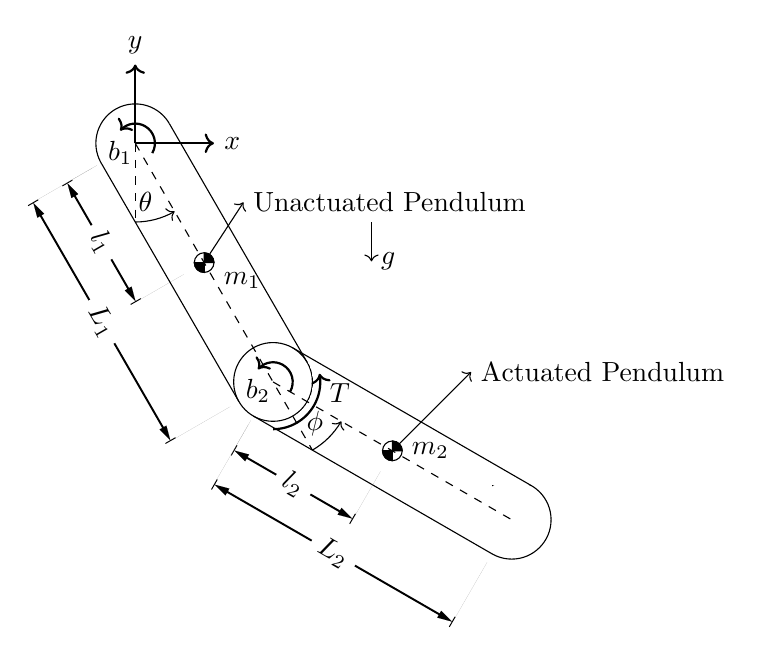
\begin{tikzpicture}[scale=0.5]

\begin{scope}
\clip [rotate=30] (-2,0) rectangle (2,2);
\draw (0,0) circle [radius=1cm];
\end{scope}

\coordinate (O) at (0,0) ;
% Second cirle middle point
\coordinate (A) at (3.5,-6.06217); 
\coordinate (B) at (3.5+6.06217,-6.06217-3.5); 
	% Lenght of pendulums are 7cm

	% Axis for underactuated Pendulum
	\draw[->,thick] (0,0) -- (2,0) node[anchor=west] {$x$};
	\draw[->,thick] (0,0) -- (0,2) node[anchor=south] {$y$};
	\draw[dashed] (0,0) -- (0,-2);
	
	%%%%%%%%%%%%%%%%%%%%%%%%%%%%%%%%%%%%%%%%%%%%%%%%%%%%%%%%%%%%%%%%%%%%%%%%%%%%%%
							%% Theta %%
	\begin{scope}
		\draw[->] (0,-2) arc (270:300:2);
		\draw (280:1.5) node {$\theta$};
	\end{scope}
	%%%%%%%%%%%%%%%%%%%%%%%%%%%%%%%%%%%%%%%%%%%%%%%%%%%%%%%%%%%%%%%%%%%%%%%%%%%%%%
	
	%%%%%%%%%%%%%%%%%%%%%%%%%%%%%%%%%%%%%%%%%%%%%%%%%%%%%%%%%%%%%%%%%%%%%%%%%%%%%%
				%% Middle line for underactuated pendulum %%
	\draw[dashed] (0,0) -- (4.5,-7.79422);
	%%%%%%%%%%%%%%%%%%%%%%%%%%%%%%%%%%%%%%%%%%%%%%%%%%%%%%%%%%%%%%%%%%%%%%%%%%%%%%
	
		
	%%%%%%%%%%%%%%%%%%%%%%%%%%%%%%%%%%%%%%%%%%%%%%%%%%%%%%%%%%%%%%%%%%%%%%%%%%%%%%
					%% Dimensions of underactuated Pendulum %%
	\dimline[line style = {line width=0.7},extension start length=-0.25, extension end length=-0.4]{(-1.732,-1)}{(-1.732+1.75,-1-3.031)}{$l_{1}$}
	
	\dimline[line style = {line width=0.7},extension start length=-0.25, extension end length=-0.25]{(-2.598,-1.5)}{(-2.598+3.5,-1.5-6.06217)}{$L_{1}$}
	
	%%%%%%%%%%%%%%%%%%%%%%%%%%%%%%%%%%%%%%%%%%%%%%%%%%%%%%%%%%%%%%%%%%%%%%%%%%%%%%

	%Long lines for underactuated pendulum
	\draw (0.8660,0.5) -- (0.866+3.5,0.5-6.06217);
	\draw (-0.8660,-0.5) -- (-0.866+3.5,-0.5-6.06217);	
	
	
	
	%%%%%%%%%%%%%%%%%%%%%%%%%%%%%%%%%%%%%%%%%%%%%%%%%%%%%%%%%%%%%%%%%%%%%%%%%%%%%%
					%% Middle circle for both pendulums %%
	\begin{scope}
		%\clip [rotate=00] (0.866+3.5,0.5-6.06217+2) rectangle (-0.866+3.5-2,-0.5-6.06217);
	\clip (A) circle [radius=1.02];
	\draw (A) circle [radius=1cm];
	\end{scope}
	
	%\draw [rotate=00] (0.866+3.5,0.5-6.06217+2) rectangle (-0.866+3.5-2,-0.5-6.06217);
	
	%%%%%%%%%%%%%%%%%%%%%%%%%%%%%%%%%%%%%%%%%%%%%%%%%%%%%%%%%%%%%%%%%%%%%%%%%%%%%%
	% Axis for lower Pendulum
	%\draw[->,thick] (3.5,-6.06217) -- (6.5,-6.06217) node[anchor=west] {$x_{2}$};
	%\draw[->,thick] (3.5,-6.06217) -- (3.5,-3.06217) node[anchor=south] {$y_{2}$};
	%\draw[dashed] (3.5,-6.06217) -- (3.5,-8.56217);
	
	% Long lines for actuated pendulum
	\draw (3.5+0.5,-6.06217+0.86602) -- (3.5+0.5+6.06217,-6.06217+0.86602-3.5);
	\draw (3.5-0.5,-6.06217-0.86602) -- (3.5-0.5+6.06217,-6.06217-0.86602-3.5);
	
	%%%%%%%%%%%%%%%%%%%%%%%%%%%%%%%%%%%%%%%%%%%%%%%%%%%%%%%%%%%%%%%%%%%%%%%%%%%%%%
							%%  Phi %%
	\begin{scope}
	\draw[->] (4.5,-7.79422) arc (300:330:2);
	
	
	\draw (3.5,-6.06217)+ (315:1.5) node {$\phi$};
	\end{scope}
	%%%%%%%%%%%%%%%%%%%%%%%%%%%%%%%%%%%%%%%%%%%%%%%%%%%%%%%%%%%%%%%%%%%%%%%%%%%%%%
	
	%%%%%%%%%%%%%%%%%%%%%%%%%%%%%%%%%%%%%%%%%%%%%%%%%%%%%%%%%%%%%%%%%%%%%%%%%%%%%%
						%% Dimensions of actuated Pendulum %%
	\dimline[line style = {line width=0.7},extension start length=-0.25, extension end length=-0.4]{(2.5,-7.79421)}{(5.53108,-9.54422)}{$l_{2}$}
	
	\dimline[line style = {line width=0.7},extension start length=-0.25, extension end length=-0.25]{(2,-8.66028)}{(8.06217,-12.1602)}{$L_{2}$}
	
	%%%%%%%%%%%%%%%%%%%%%%%%%%%%%%%%%%%%%%%%%%%%%%%%%%%%%%%%%%%%%%%%%%%%%%%%%%%%%%

	
	%%%%%%%%%%%%%%%%%%%%%%%%%%%%%%%%%%%%%%%%%%%%%%%%%%%%%%%%%%%%%%%%%%%%%%%%%%%%%%
							%% Circle at the bottom %%
	\begin{scope}
	\clip [rotate=00] (3.5+0.5+6.06217+2,-6.06217+0.86602-3.5) rectangle ((3.5-0.5+6.06217,-6.06217-0.86602-3.5-2);
	\draw (B) circle [radius=1cm];
	\end{scope}
	%%%%%%%%%%%%%%%%%%%%%%%%%%%%%%%%%%%%%%%%%%%%%%%%%%%%%%%%%%%%%%%%%%%%%%%%%%%%%%

	
	%%%%%%%%%%%%%%%%%%%%%%%%%%%%%%%%%%%%%%%%%%%%%%%%%%%%%%%%%%%%%%%%%%%%%%%%%%%%%%
					%% Middle line for actuated pendulum %%
	\draw[dashed] (3.5,-6.06217)--(3.5+6.06217,-6.06217-3.5);
	%%%%%%%%%%%%%%%%%%%%%%%%%%%%%%%%%%%%%%%%%%%%%%%%%%%%%%%%%%%%%%%%%%%%%%%%%%%%%%
		
	%%%%%%%%%%%%%%%%%%%%%%%%%%%%%%%%%%%%%%%%%%%%%%%%%%%%%%%%%%%%%%%%%%%%%%%%%%%%%%
				%% Centroid symbol for underactuade pendulum %%
	\draw (1.75,-3.0310) circle [radius=0.25cm];
	\draw (1.75-0.25,-3.0310) -- (1.75+0.25,-3.0310)  node[below right]{$m_{1}$};`
	\draw (1.75,-3.0310+0.25) -- (1.75,-3.0310-0.25);
	\filldraw[fill=black,draw=black] (1.75,-3.0310) -- (1.75+0.25,-3.0310)
		arc[start angle = 0, end angle = 90, radius = 0.25] -- cycle;
		
	\filldraw[fill=black,draw=black] (1.75,-3.0310) -- (1.75-0.25,-3.0310)
	arc[start angle = 180, end angle = 270, radius = 0.25] -- cycle ;
	%%%%%%%%%%%%%%%%%%%%%%%%%%%%%%%%%%%%%%%%%%%%%%%%%%%%%%%%%%%%%%%%%%%%%%%%%%%%%%
	
	%%%%%%%%%%%%%%%%%%%%%%%%%%%%%%%%%%%%%%%%%%%%%%%%%%%%%%%%%%%%%%%%%%%%%%%%%%%%%%
				%% Centroid symbol for actuaded pendulum %%
	\draw (6.53108,-7.81217) circle [radius=0.25cm];
	\draw (6.53108-0.25,-7.81217) -- (6.53108+0.25,-7.81217)  node[right]{$m_{2}$};
	\draw (6.53108,-7.81217+0.25) -- (6.53108,-7.81217-0.25);
	\filldraw[fill=black,draw=black] (6.53108,-7.81217) -- (6.53108+0.25,-7.81217)
	arc[start angle = 0, end angle = 90, radius = 0.25] -- cycle;
	
	\filldraw[fill=black,draw=black] (6.53108,-7.81217) -- (6.53108-0.25,-7.81217)
	arc[start angle = 180, end angle = 270, radius = 0.25] -- cycle ;
	%%%%%%%%%%%%%%%%%%%%%%%%%%%%%%%%%%%%%%%%%%%%%%%%%%%%%%%%%%%%%%%%%%%%%%%%%%%%%%
	
	% Torque Input
	%\draw[->,thick] (3.5,-7.5) to [bend right] (5.25,-4.76314) node[right]{$T$}; 
	\draw[->,thick] (A) +(0,-1.2) arc (270:370:1.2) node[below right] {$T$};
	
	
	% Damping in bearings
	\draw[->,thick] (0.433,-0.25) arc (330:500:0.5) node[below] {$b_{1}$};
	
	% Damping between motor rotor and stator 
	\draw[->,thick] (A)+(0.433,-0.25) arc (330:500:0.5) node[below] {$b_{2}$};
	
	% Direction of gravity
	\draw[->] (6,-2)--(6,-3) node[right]{$g$};
	
	% Labels for pendulums
	\draw[->] (1.75,-3.0310)--(2.75,-1.5) node[right]{Unactuated Pendulum};
	\draw[->] (6.53108,-7.81217)--(8.53108,-5.81217) node[right]{Actuated Pendulum};
	
	
\end{tikzpicture}
		\caption{Free Body Diagram of the Double Pendulum}
		\label{fig:doublePen}
	\end{figure}

	The approach taken to derive the mathematical model of the robotic gymnast will be discussed in this section. It is presented to allow the reader to understand parameters mentioned in the report. The swing-up of the robotic gymnast consist of non-linear behaviour and is require to fully derive the dynamics of the system. The strenuous mathematical steps are removed from the reader, which is provided in Appendix A, and a summary of the motivation and paradigm approach to the derivation is provided.

	The robotic gymnast is modeled as two pendulums connected together with a hinge, where each pendulum is modeled as having their mass distributed arbitrary along their axis. There is a torque actuating the lower pendulum seen in Figure \ref{fig:doublePen} and friction is modeled as proportional to the angular velocity of the pendulums. The friction that develops at the hinge is proportional to the relative motion of the actuated pendulum and non-actuated pendulum. The angle, $\phi$ was purposefully chosen relative to $\theta$ to ease the identification of this friction. Figure \ref{fig:doublePen} displays the free body diagram of the robotic gymnast.
	
	Deriving the equation of motion of the robotic gymnast can be approached using different methods, but by exploring the system it can be shown that the system's energy is easily defined. The energy in the system is the potential energy of the 2 pendulums, the rotational kinetic energy of the non-actuated pendulum and the velocity- and rotational kinetic energy of the actuated pendulum. The Euler-Lagrange equation is chosen to derive the differential equation describing the system dynamics because of the easily defined energy. Using the Euler-Lagrange equation leads to the condense equations shown in (\ref{eq:condense1}) and (\ref{eq:condense2}),
	\begin{equation} \label{eq:condense1}
		d_{11}\ddot{\theta}+d_{12}\ddot{\phi} + h_{1} + \psi_{1} = 0
	\end{equation}
	\begin{equation} \label{eq:condense2}
			d_{21}\ddot{\theta} + d_{22}\ddot{\phi} + h_{2} + \psi_{2} = \tau
	\end{equation}
	where
		\begin{equation} \label{eq:d11}
	d_{11} = I_{a} + I_{b} + m_{2}(L_{1}^2 + l_{2}^2+2L_{1}l_{2}\cos(\phi))
	\end{equation}
		\begin{equation} \label{eq:d12}
	d_{12} = I_{b} +m_{2}(l_{2}^2 L_{1}l_{2}\cos(\phi))
	\end{equation}
		\begin{equation} \label{eq:h1}
	h_{1} = -m_{2}L_{1}l_{2}\sin(\phi)\dot{\phi^2}-2m_{2}L_{1}l_{2}\sin(\phi)\dot{\phi}\dot{\theta}
	\end{equation}
		\begin{equation} \label{eq:psi1}
	\psi_{1} = (m_{2}l_{1}+m_{2}L_{1})g\cos(\theta) + m_{2}l_{2}g\cos(\theta+\phi)
	\end{equation}
		\begin{equation} \label{eq:d21}
	d_{21}= I_{b}+m_{2}(l_{2}^2+L_{1}l_{2}\cos(\phi))
	\end{equation}
		\begin{equation} \label{eq:d22}
	d_{22}= I_{b}+ m_{2}l_{2}^2
	\end{equation}
		\begin{equation} \label{eq:h2}
	h_{2}= m_{2}L_{1}l_{2}\sin(\phi)\dot{\theta^2}
	\end{equation}
		\begin{equation} \label{eq:psi2}
	\psi_{2}= m_{2}l_{2}g\cos(\theta+\phi)
	\end{equation}
	
	
	
	The equation of motion for the robotic gymnast is very non-linear containing multiple terms of squared angular velocities and cosine functions. These non-linearities is hidden in the in the $\psi$ and $h$ terms. The non-linearities can be linearised around a working point, but during the swing-up of the robotic gymnast they must be taken into account.
 
	
	
	\section{Swing Up of the Double Pendulum}
	% WHAT you are going to present in this chapter/section
	% WHY you are presenting it, and
	% HOW you are going to present it	
	The swing up of the robotic gymnast is done by the non-linear feedback control system. For the robotic gymnast to swing from the stable equilibrium position to the unstable equilibrium position the feedback control must incorporate the non-linearities of the system. How these non-linearities of the system is incorporated and the design paradigm of the approach will be explained in following text.
	
	It has been shown that it is not possible to linearise the dynamics of the gymnast by means of static state feedback and non-linear transformation \cite{murray}, but it is possible to achieve a linear response from one of the state variables by implementing a non-linear feedback. This non-linear feedback is the partial feedback linearisation.
	
	Collocated linearisation is a form of partial feedback linearisation where a non-linear control input $\tau$ is used to linearise the response of the actuated pendulum. By analysing equation (\ref{eq:collocated_lin2}), the input $\tau$ is chosen to cancel all the non-linearities of the system and add an additional outer loop control input $v_{2}$. This outer loop control input can be selected to force the actuated pendulum to follow a desired trajectory \cite{spong_swingup}. The derivation of the collocated linearisation is shown in appendix C.
	
	\begin{equation} \label{eq:collocated_lin1}
	d_{11}\ddot{\theta} + h_{1} + \psi_{1} = -d_{12}v_{2}
	\end{equation}
	\begin{equation} \label{eq:collocated_lin2}
	\ddot{\phi} = v_{2}
	\end{equation}
	
	The ability to control the actuated pendulum to follow a desired trajectory, provides the possibility to increase the energy of the system if the correct trajectory is chosen. The increase of energy in the system will cause the pendulums to rise from their stable equilibrium position and thus start swinging upwards. The desired trajectory for ${\phi}$ is chosen as equation (\ref{eq:desired_phi}) determined by W.Spong in \cite{spong_swingup}.
	\begin{equation} \label{eq:desired_phi}
	\phi^{d} =  \alpha \arctan(\dot{\theta})
	\end{equation}
	
	The outer loop control input, $v_{2}$, is chosen as 
	\begin{equation} \label{eq:v2}
	v_{2} = K_{p}(\phi^{d}-\phi)-K_{d}\dot{\phi}
	\end{equation}
	
	The desired trajectory is chosen to increase the energy in the system, approach is to allow the actuated pendulum swing in phase with the non-actuated pendulum. By this approach the energy of the actuated pendulum is transferred to the non-actuated pendulum \cite{spong_swingup}. Appendix E shows how this approach is expected to work.

	Returning to the desired trajectory of $\phi$, the coefficient $\alpha$ constrains the actuated pendulum to stay within a interval of $ \phi \in [-\alpha,\alpha] $ \cite{spong_swingup}. This provides better control over the system to stay within the null controllability region when the system reaches the unstable inverted position.
	
		  
	\section{Balancing of the Double Pendulum}
	% WHAT you are going to present in this chapter/section
	% WHY you are presenting it, and
	% HOW you are going to present it
	
	Provided the robotic gymnast is within the region of controllability, a balancing controller is required to bring the system to the unstable equilibrium position. The design approach is based on the premises that the swing-up controller will swing the robotic gymnast within the region of controllability where the balancing controller will steer the robotic gymnast to balancing.
	
	%The balancing of the gymnast will be achieved by catching the gymnast when the swing-up control algorithm has brought the gymnast to the null controllability region. The null controllability region is the set of states that can be steered to inverted unstable equilibrium position in a fixed time with a constrained control input \cite{null_controllability}.
	The independent parameters, $\phi$ and $\theta$, will be condensed from now on as a vector describes as $$ \vec{q} = 
	\begin{bmatrix}
	\theta \\
	\phi
	\end{bmatrix}
	$$
	
	The system can be approximated as a linear system when in the vicinity of the unstable equilibrium position. The system is thus linearised at $$\vec{Q_{s}} = [\vec{q_{s}},\dot{\vec{q_{s}}},\ddot{\vec{q_{s}}}]^{T}=[\pi,0,0,0,0,0]$$ the unstable equilibrium position using the Taylor Series Expansion shown in detail in Appendix B. This linearised model can than be written in the state space form to implement a feedback gain. The state space variables are chosen as $\Delta{\vec{q}}$ and $\Delta{\dot{\vec{q}}}$ which results in the state space representation as:  $$ \dot{\vec{q}} = \boldsymbol{A}\Delta{\vec{q}} + \boldsymbol{B}u $$ and $$ \vec{y} = \boldsymbol{D}\Delta{\vec{q}} + \boldsymbol{0}u $$.
	
	The linearised system remains a coupled system which results that the quadratic eigenvalue problem is required to be solved to identified the poles of the system. The solved quadratic eigenvalue problem results in the following poles from the system parameters in Table \ref{table:system_param}.
	$$
	\vec{s} = 
	\begin{bmatrix}
		-8.2 \\
		-4.2	\\
		8.2 \\
		4.2 \\
		
	\end{bmatrix}
	$$
	
	The poles of the system are pairs of positive and negative real poles that indicates an unstable system. This is expected due to the system being linearised in the unstable equilibrium position. When the linearised system is at rest, any disturbance will result in a theoretically infinite growth of the state variables, but this behaviour can be controlled by introducing feedback. \\
	\\
	These poles will be moved to the desired position by using the method of dominant poles. The method of dominate poles chooses a pair of the poles for the closed-loop system and select the other open-loop poles to have real parts. This allows the higher-order system response to be characterised as a second-order response \cite{textbook}. The linearised model already has 2 negative real poles which is chosen to stay the same. The real positive poles were selected based on the following specifications.
	
	These specification was selected on increasing the null controllability region with a low settling time. Due the approximation of the linearised model the null controllability region may be larger than the derived sized \cite{simple_null_controllability}. 
	
	
	\section{Null Controllability Region}
	
	The null controllability region is the set of states, $\vec{x_{0}} \in \Re $ which can be steered with a constrained input in finite time to the origin. This region is important because it provides the boundary where the linear controller is capable of catching the swinging gymnast. The possibility exist that the set might be larger due to approximation in the working point during linearisation of the system \cite{simple_null_controllability}. 
	
	To determine the null controllability region requires a transformation into independent equation and followed by a technique describe in .. . The linearised system are coupled and due to damping effect results in a quadratic eigenvalue problem. The de-coupling can be done by using phase-synchronisation describe in \cite{independent_eqaution} and shown in Appendix XXX. The phase-synchronisation results in 2 transformed eigenvalues, $\lambda'$ and creates 2 damping ratio's, $\zeta'$ to from two independent second-order equations. The values for $\lambda'$'s and $\zeta'$'s is as follows: $$ \boldsymbol{\lambda} = [ ]^{T} $$ $$ \boldsymbol{\zeta} = []^{T} $$
	
	From these two independent second-order equations the null controllability region can be determine using time-reversal describe in \cite{null_controllability}.
	
	$$ \vec{x} = e^{\boldsymbol{A}t}\vec{x_{0}} + \int_{t_{1}}^{t_{2}} e^{-\boldsymbol{A}t}\boldsymbol{B}u dt $$ 
	
	$$\mathcal{R} = {-\int_{-\infty}^{0} e^{A\tau}bsgn(c'e^{A\tau})d\tau }  $$
	
	$$\mathcal{C} $$ 
	
	
	\section{System Identification}
	
	%WHAT you are going to present in this chapter/section
	%WHY you are presenting it, and
	%HOW you are going to present it?
	
	The system identification tests are done to determine the characteristics that describe the behavior of the system. These characteristics include the damping ratio's and natural frequencies of the system around the unstable equilibrium position. The system are described by 2 independent parameters, $\theta$ and $\phi$ which defines the position of the non-actuated and actuated pendulums. The system is thus a 2 degree of freedom (2DOF) system and it is expected to contain 2 natural frequencies each accompanied by a damping coefficient.
	
	The first natural frequency of the system is determine by inspecting the response of the system when starting at a initial condition and keeping $\phi = \SI{0}{rad}$ constant throughout the response. This was done by using a lightweight PVC pipe that has negligible effect on the weight of the system. The actuated pendulum and non-actuated pendulum are constrained to this pipe to ensure the 2 pendulums stay in-line with each other and thus ensuring $\phi = \SI{0}{rad}$. The response of the system is shown in Figure \ref{fig:q1_response} starting at a initial condition of roughly $\theta = \frac{\pi}{2}$. The accuracy of the initial conditions is of little importance, but the initial condition must allow the response to contain a few oscillation to accurately determine the parameters of interest. The second natural frequency is determined by analysing the response of the system when $\phi$ starts at a initial condition and keeping $\theta = \SI{0}{rad}$ throughout the response. This was accomplished by constraining the non-actuated pendulum using hard stops. Figure \ref{fig:q2_response} shows the measured response of the system when $\phi$ starts at a initial condition and keeping $\theta$ constant.%ith with an approximated response that is determined by the parameters shown in Table \ref{table:system_response_prop}.
	
	The natural frequencies of the system is identified by inspecting the frequency content of the time-domain responses. The frequency content of the initial condition responses of both experiments are shown in Figure \ref{fig:fft_system_response}, by applying the Fast Fourier Transform (FFT) algorithm to the time-domain signals. The FFT indicates the natural frequencies by the predominant peaks across the frequency spectrum which are tabulated in Table \ref{table:system_characteristic}.
	
	The responses shown in Figure \ref{fig:q1_response} and \ref{fig:q2_response} are decaying with time and this decaying behaviour can be modeled by the following equation: $$\tau(t) = -\zeta \omega_{n} t$$ Where $\omega_{n}$ is the natural frequency of the system and $\zeta$ the damping ratio of the system. The natural frequencies of the system has already been determined and thus linear regression can be used to determine the best $\zeta$ that will fit the measured data. The decaying functions are shown in Figure \ref{fig:q1_response} and \ref{fig:q2_response} with the best fit $\zeta$ values shown in Table \ref{table:system_characteristic}. It is visible from the responses that the damping ratio changes when the response are nears steady state. This change of damping ratio is neglible due to the controllers being implement are robust to changes in $\zeta$.
	
	The input to the system is the torque delivered by the motor and the magnitude and direction is determined by the control laws. The model describing the system in equation \ref{eq:condense2} assumes the torque delivered to the system is instantaneously available. This is inaccurate due to the DC motor model describing the torque delivered by the model when applying a DC voltage. The input that the motor will be receiving is a Pulse-Width-Modulated (PWM) signal to represent a DC voltage.
	
	Experiments were done to determine the relationship between the duty-cycle of the PWM signal and the torque delivered by the motor. These experiments are done by incrementing the duty-cycle of the PWM signal that the motor receives when the shaft is kept fix against a hard-stop. The motor-driver that controls the motor has a feedback pin that provides a proportional current of $\frac{1}{375}$ of the current flowing through the motor. This proportional current is allowed to flow through a known resistor. The voltage across the resistor is measured and provides a indication of the current flowing through the motor. The mean value of the voltage measured on the oscilloscope is taken and mapped backwards to determine the current. Figure \ref{fig:dutycycle_vs_current} shows the measured data with a line of best fit. It is clear that there exist a linear relationship between the duty-cycle of the PWM signal and the torque the motor can provide.
	
	\begin{table}[]
		\centering
		\begin{tabular}{|c|c|c|c|}
			\hline
			 System Characteristic & Mean & Standard Deviation\\
			\hline
			\hline
			$f_{1}$ & \SI{3.93}{Hz} &  \\
			\hline
			$f_{2}$ & \SI{3.62}{Hz} & 0.04029 \\ 
			\hline
			$\zeta_{1}$ & $1.6931 \cdot10^{-5}$ & $4.823\cdot 10^{-6}$
			 \\
			\hline
 			$\zeta_{2}$ & $5.85184 \cdot 10^{-5}$ & \\
 			\hline
	\end{tabular}
	\caption{System Characteristic \& their Statistical Properties from 10 Experiments}
	\label{table:system_characteristic}
	\end{table}

	
	\begin{figure}[h]
		\centering
		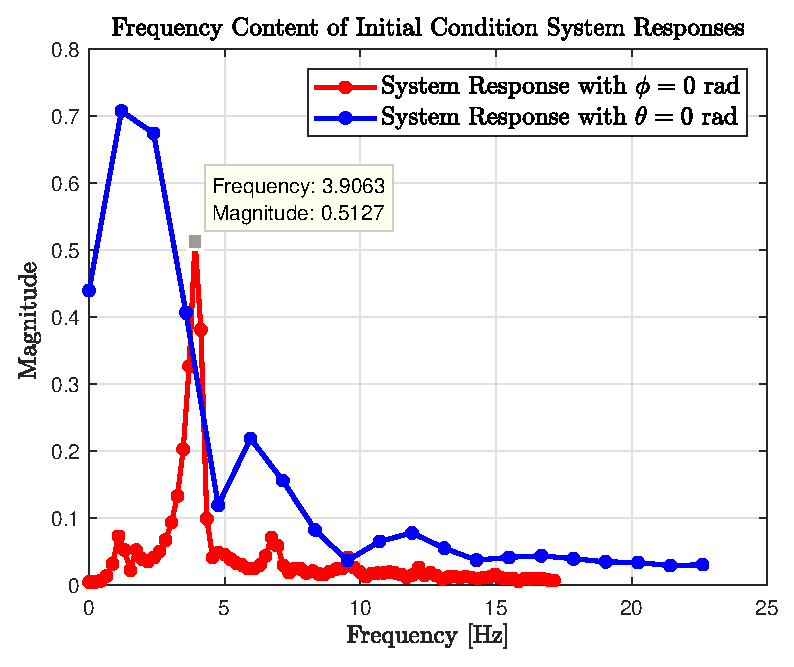
\includegraphics[scale=1]{FFT_system.eps}
		\caption{Frequency Content of Time-Domain Initial Condition Responses}
		\label{fig:fft_system_response}
	\end{figure}
	
	Figure \ref{fig:q1_response} shows the decaying function with properties that are shown in Table \ref{table:system_response_prop} and it is visible that the calculated values provides a acceptable approximation of the measured data.
	
	\begin{figure}[h]
		\centering
		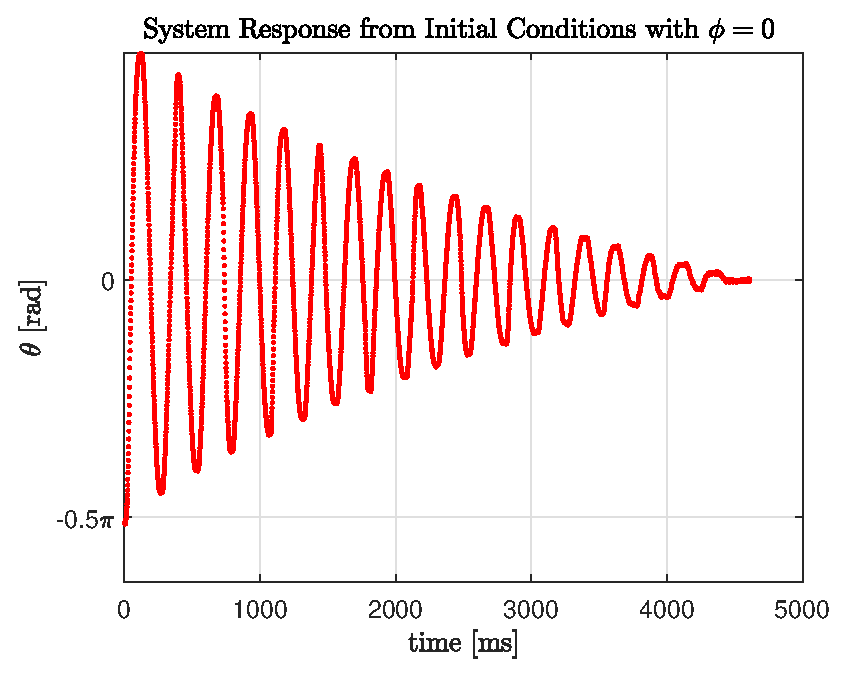
\includegraphics[scale=1]{q1_initial_response.eps}
		\caption{Initial Condition System Response while $ \phi = \SI{0}{rad} $ }
		\label{fig:q1_response}
	\end{figure}
		
	
	\begin{figure}[h]
		\centering
		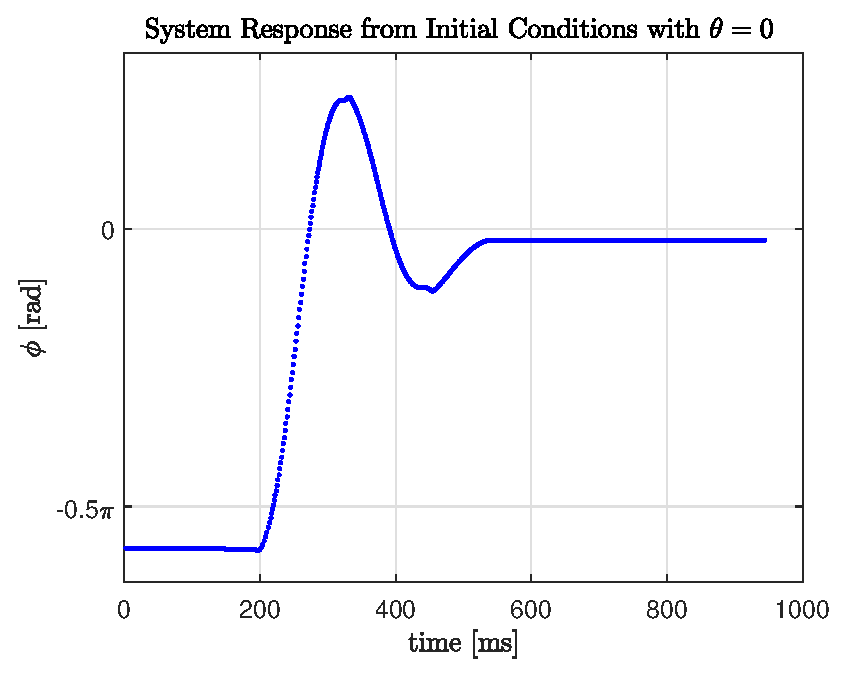
\includegraphics[scale=1]{q2_initial_response.eps}
		\caption{Initial Condition System Response while $ \theta = \SI{0}{rad} $ }
		\label{fig:q2_response}
	\end{figure}

	\begin{figure}[h]
	\centering
	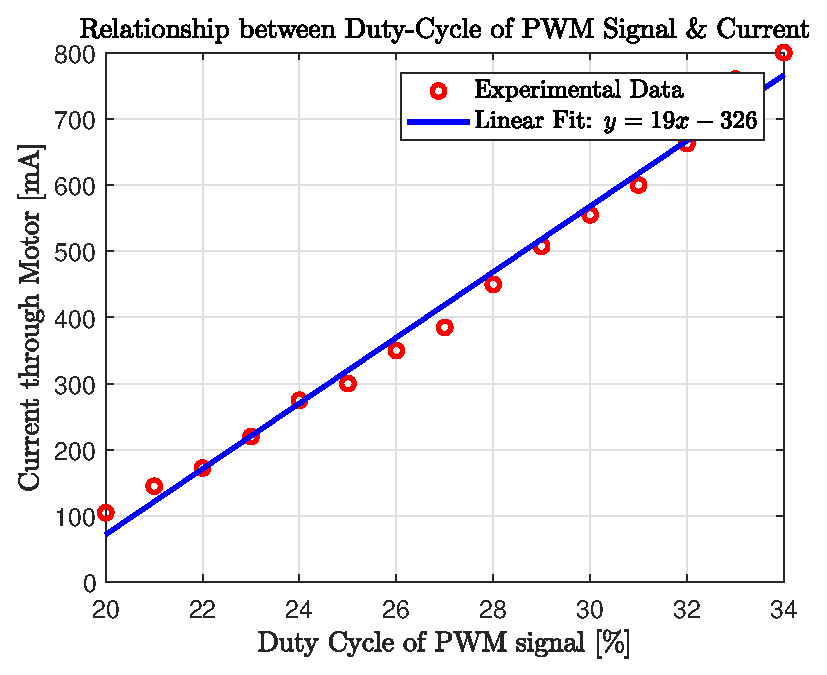
\includegraphics[scale=1]{dutycycle_vs_current.eps}
	\caption{Relationship between Duty-Cycle of PWM Signal and Current through Motor}
	\label{fig:dutycycle_vs_current}
\end{figure}


	

	
	\section{Simulating the Double Pendulum}
	%WHAT you are going to present in this chapter/section
	%WHY you are presenting it, and
	%HOW you are going to present it?
	
	The process of simulating the robotic gymnast and ensuring the simulation provide a true representation of the system is discussed. Simulation of the robotic gymnast plays a important role during the design process. It allows the designer to develop a intuition for the system, enables the verification of dynamics and the creation of specification for the mechanical design. It will be presented by discussing how the simulation is a true representation of the system, how design specifications were determined and the influence of these parameters.

	Simulation of the gymnast was done using MATLAB Simulink. The differential equations were implemented shown in equations \ref{eq:condense1} and \ref{eq:condense2} and non-linearities such as saturation of the motor, gearbox backlash and quantisation of sensory data were implemented to represent a true system. Verification of successful implementation of the differential equations were done by removing all non-linearities created by hardware and removing the damping effects. When the system is given a initial condition it is expected that the mechanical energy in the system will remain constant. This behaviour is shown in Figure \ref{fig:mechanical_energy} and verifies the correct implementation of the mathematical model. 
	
	System characteristic values such as inertia and pendulum lengths were unavailable during simulations owning to the mechanical design that was incomplete. Initially the system variables such as inertia and pendulum lengths were selected from values that represented a physical system. The accuracy of these values were credible being taken from a previous physical model. From these simulation motor specification could be determine and the influence of system variables could be analysed. System variables that influenced the ability of the control system to swing the robotic gymnast is the ratio of the inertia's of the 2 pendulums, $\frac{I_{b}}{I_{a}}$. It was witnessed that the control system took significantly longer to swing the gymnast to the upright position between a ratio of 0.5 and 1. This is due to the amount of energy that the actuated pendulum can transfer is much less, and thus requires longer time to swing up.
	
	Damping coefficients were given a realisitic value
	
	Once the mechanical system was designed and manufactured and the system identification was completed the true system parameters could be used in the simulation. These system parameters are shown in Table \ref{table:system_param}. Using the system parameters shown in Table \ref{table:system_param} the natural frequencies of the linearised system, the feedback gain matrix for the balancing control and the gain constants for the swing-up control were determined. 
	
	Figure \ref{fig:swingup&balance} shows the simulated swing-up and balance of the double pendulum. As discussed in the Swing-up Controller section the $\alpha$ value controls the relative angle between actuated pendulum and the non-actuated pendulum. This $\alpha$ value is decreased throughout the swing-up of the robotic gymnast to ensure the robotic gymnast can be approximated as a single pendulum to allow the linear controller to catch the swinging pendulums.
	
		
	\begin{figure}[h]
		\centering
		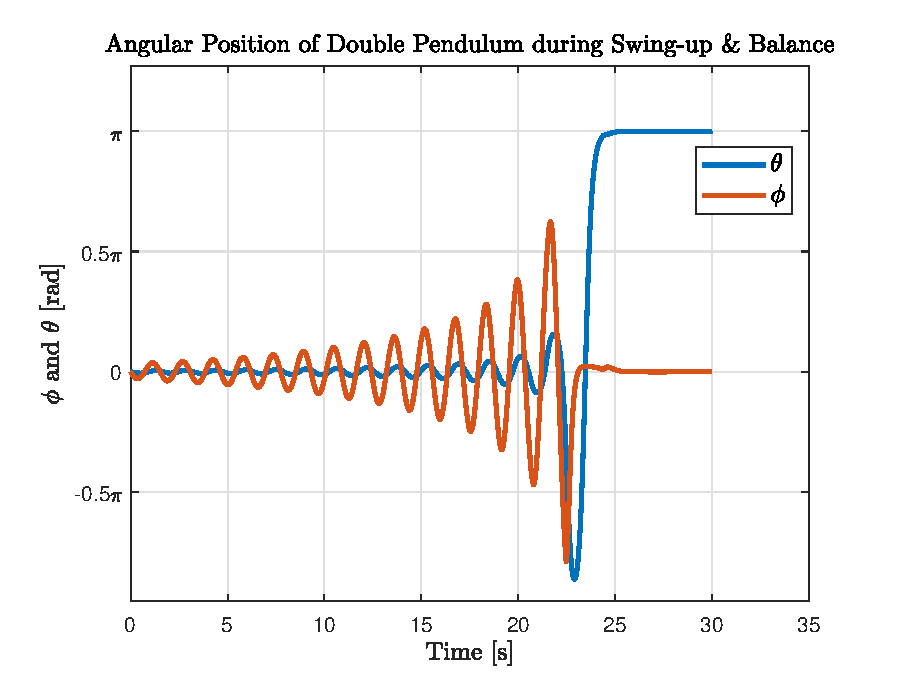
\includegraphics[scale=1]{swingup_balance.eps}
		\caption{Swing-up \& Balancing of Robotic Gymnast in Simulation }
		\label{fig:swingup&balance}
	\end{figure}
	
	
	Figure \ref{fig:balancing} shows the response of the system when given a initial condition that is within the region of controllability in which the balancing controller moves the system to the unstable equilibrium position. The response shows that the balancing controller is capable of balancing the robotic gymnast.
	
	
		\begin{table}[]
		\centering
		\begin{tabular}{|c|c|}
			\hline
			System Parameter & Value \\
			\hline
			\hline
			$L_{1}$ & \SI{0.235}{m} \\
			\hline
			$L_{2}$ & \SI{0.245}{m} \\ 
			\hline
			$I_{A}$ & \SI{0.0265}{kg\cdot m^2}\\
			\hline
			$I_{B}$ & \SI{0.0221}{kg\cdot m^2}\\
			\hline
			$m_{1}$ & \SI{0.5763}{kg}\\
			\hline
			$m_{2}$ & \SI{0.4928}{kg} \\
			\hline
			$l_{1}$ & \SI{0.235}{m}\\
			\hline
			$l_{2}$ & \SI{0.245}{m}\\
			\hline
		\end{tabular}
		\caption{System Parameters}
		\label{table:system_param}
	\end{table}
	
	\subsection{Feedback Control for Balancing Controller}
	
	The balancing controller is responsible for catching the swinging pendulums and bring the system to rest at the unstable equilibrium position. The balancing controller is required to bring the system from a initial condition in the vicinity of the unstable equilibrium position to reach steady state of balancing in the unstable equilibrium position. The system can be portrayed as seen in Figure \ref{fig:linearSys}.
	
	The system will have unstable poles when in the vicinity of the unstable equilibrium position as shown in Table \ref{table:poles_of_system}. The feedback gain matrix must move these poles to a stable location with desired system response properties.
	
	The desired system response 
	
	
	
	
	\subsection{Feedback Control for Swing-up Controller}

	
	\section{Why Designing in the Continuous Time Domain is Sufficient}
	
	\section{Mechanical Design of the Double Pendulum}
	%WHAT you are going to present in this chapter/section
	%WHY you are presenting it, and
	%HOW you are going to present it?
	
	Translating the mathematical model into a true physical representation it is important that the assumptions made during the derivation of the model remains in the physical model. These assumption include planar translation, rigid body dynamics and friction that is proportional to angular velocity. The section will discuss how the mechanical design was done according to these assumptions.
	
	%These assumptions was implemented by using contact ball bearings
	\newpage
	\section{Electronic Design of the Double Pendulum}
	
	\subsection{System Description}
	
	% Show block diagram of the system and explain the functioning og the system
	\begin{figure}[h]
		\centering
		\usetikzlibrary{shadows,arrows}
% Define the layers to draw the diagram
\pgfdeclarelayer{background}
\pgfdeclarelayer{foreground}
\pgfsetlayers{background,main,foreground}

% Define block styles  
\tikzstyle{block}=[draw, fill=blue!20, text width=7.0em, text centered,
minimum height=1.5em,drop shadow]
\tikzstyle{blocks} = [block, rounded corners, drop shadow]
\tikzstyle{texto} = [above, text width=6em, text centered]
\tikzstyle{linepart} = [draw, thick, color=black!50, -latex', dashed]
\tikzstyle{line} = [draw, thick, color=black!50, -latex']
\tikzstyle{ur}=[draw, text centered, minimum height=0.01em]

% Define distances for bordering
\newcommand{\blockdist}{1.3}
\newcommand{\edgedist}{1.5}

\newcommand{\external}[2]{node (e#1) [blocks]
	{External 12V Supply\\{\scriptsize\textit{#2}}}}

\newcommand{\regulator}[2]{node (r#1) [blocks]
	{Voltage Regulation\\{\scriptsize\textit{#2}}}}

\newcommand{\uC}[2]{node (uC#1) [blocks]
	{$\mu$Controller\\{\scriptsize\textit{#2}}}}

\newcommand{\uart}[2]{node (uart#1) [blocks]
	{PC UART Interface\\{\scriptsize\textit{#2}}}}

\newcommand{\prog}[2]{node (prog#1) [blocks]
	{Programming / Debug Interface\\{\scriptsize\textit{#2}}}}

\newcommand{\motor}[2]{node (motor#1) [blocks]
	{Motor\\{\scriptsize\textit{#2}}}}

\newcommand{\sigcond}[2]{node (sigcond#1) [blocks]
	{Signal Conditioning\\{\scriptsize\textit{#2}}}}

\newcommand{\encdig}[2]{node (encdig#1) [blocks]
	{Digital Logic Circuit\\{\scriptsize\textit{#2}}}}

\newcommand{\pc}[2]{node (pc#1) [blocks]
	{PC\\{\scriptsize\textit{#2}}}}

\newcommand{\physical}[2]{node (physical#1) [blocks]
	{Physical Model\\{\scriptsize\textit{#2}}}}

\newcommand{\motordriver}[2]{node (motordriver#1) [blocks]
	{Motor Driver\\{\scriptsize\textit{#2}}}}

\newcommand{\digitlogic}[2]{node (digitlogic#1) [blocks]
	{Digital Logic Circuit\\{\scriptsize\textit{#2}}}}

\newcommand{\encoder}[2]{node (encoder#1) [blocks]
	{Hall Effect Encoder\\{\scriptsize\textit{#2}}}}
% Draw background
\newcommand{\background}[5]{%
	\begin{pgfonlayer}{background}
		% Left-top corner of the background rectangle
		\path (#1.west |- #2.north)+(-0.5,0.5) node (a1) {};
		% Right-bottom corner of the background rectanle
		\path (#3.east |- #4.south)+(+0.5,-0.25) node (a2) {};
		% Draw the background
		\path[fill=yellow!20,rounded corners, draw=black!50, dashed]
		(a1) rectangle (a2);
		\path (a1.east |- a1.south)+(0.8,-0.3) node (u1)[texto]
		{\scriptsize\textit{Unidad #5}};
\end{pgfonlayer}}

\newcommand{\transreceptor}[3]{%
	\path [linepart] (#1.east) -- node [above]
	{\scriptsize Transreceptor #2} (#3);}


\begin{tikzpicture}[scale=0.7,transform shape]

% Draw diagram elements
\path \external {1}{DC Power Supply};
\path (e1.east)+(2.0,0.0) \physical{1}{Potentiometer};
\path (e1.south)+(0.0,-1.5) \regulator{1}{5V, 3.3V};
\path (r1.south)+(0.0,-1.5) \uC{1}{ARM M0 STM32F030C6};

% PC 
\path (e1.west)+(-2.5,0) \pc{1}{};

% PC UART Interface
\path (r1.west)+(-6,0) \uart{1}{FT230XS};

%Programming/Debug Interface
\path (r1)+(-4.05,0) \prog{1}{Serial Wire Debug};

%Signal Conditioning
\path (uC1.east)+(2.0,0) \sigcond{1}{OPA342 OpAmp};

%JK Flipflops
\path (uC1.west)+(-2.0,-3.0) \encdig{1}{J-K Flipflop \& Nor's};

% Motor
\path (uC1.south) + (0,-5) \motor{1}{DC Brushed Motor};

% Digital Logic: Logic Level Convertes
\path (uC1.south) + (0,-2) \digitlogic{1}{Logic Level Converters \&  Direction Control};

% Motor Driver
\path (digitlogic1.east)+(2.0,0) \motordriver{1}{MC33887};

%Hall Effect Enconder
\path (encdig1.south)+ (0,-1.8) \encoder{1}{Mounted On Motor};




% Draw arrows between elements
\path [line] (e1.south) -- node [above] {} (r1);
\path [line] (r1.south) -- node [above] {} (uC1);

% uC to UART
\path [line] (uC1.west) -| node [below] {} (uart1);

% uC to Programming/Debug Interface
\path [line] (uC1.west)+(0,0.2) -| node [below]{}(prog1); 

% JK FlipFlops
%\path [line] (uC1.west)+(0,-0.2) -| node [above]{}(encdig1); 

\draw[->] (encdig1) |- ([yshift=-0.2cm]uC1.west);


\path [line] (sigcond1.west) -- node[right]{}(uC1);

\path [line] (physical1.south) -- node[above]{}(sigcond1);

% Motor Driver to signal Conditioning
\path [line] (motordriver1.north) -- node[below]{}(sigcond1);

% PC UART Interface -> PC
\path [line] (uart1.north) |- node[left]{}(pc1);

% Programming/Debug Interfac -> PC
\path [line] (prog1.north) -- node[below]{}(pc1);

% Motor Driver -> Motor
\path [line] (motordriver1.south) |- node[right]{}(motor1); 

% Microcontroller -> Digitical logic
\path [line] (uC1.south) -- node[above]{}(digitlogic1);

\path [line] (digitlogic1.east) -- node[left]{}(motordriver1);


\path [line] (encoder1.north) -- node[below]{}(encdig1);


\path [line] (motor1.west) -- node[right]{}(encoder1);

\begin{pgfonlayer}{background}
\path (uart1.west -| physical1.east) node (a) {};
\path (motor1.south -| physical1.south)+(+0.5,-0.3) node (b) {};
\path (digitlogic1.south |- motor1.east)+(+0.5,0.5) node (c) {};

\path[fill=yellow!20,rounded corners, draw=black!50, dashed]
([xshift=-0.5cm,yshift=1cm]uart1.west) rectangle ([xshift=0.5cm,yshift=-2cm]motordriver1.east);           
\path (digitlogic1.north west)+(-0.2,0.2) node (a) {};

\end{pgfonlayer}

\path ([xshift=-4.5cm,yshift=-0.5cm]encdig1.south) node (meep) {PCB Boundary};

%\path (wa.south)+(0,-\blockdist/5) node (meep) {System Boundary};


\end{tikzpicture}
		\caption{Electronic System Overview}
		\label{fig:electronicSystemOverview}
	\end{figure}
	
	
	Figure \ref{fig:electronicSystemOverview} provides/yields a system overview and how the different parts functions together. The micro-controller receives the different signals that has been correctly conditioned from supporting circuitry to interpret the dynamics of the system. From the observed condition it is able to output the correct signals to instruct the next command.
	
	The digital logic circuit that consist of logic level converters acquires the signal from the micro-controller and performs signal conditioning to interface with the motor driver and determines the correct direction to rotate the motor. 
	
	The motor driver controls the DC brushed motor based of the digital signals and provides a proportional feedback current that is fed/deliver to buffer.
	
	The motor contains a encoder that indicates the direction and position of the rotor through digital signals that is sent through a digital logic filter to retrieve only critical information from the encoder signals. 
	
	The physical model contains a potentiometer that measures the non-actuated pendulums angle and is sent to the buffer.
	
	The microcontroller will use the UART interface as it's data acquisition protocol to send the necessary information to the computer. 
	
	The micro-controller is programmed using the Serial Wire Debug (SWD) protocol to transfer the binaries from the computer.
	
	Power is provided using a external 12V power-supply, which will power the motor, but also using a regulator to down convert/step to a 5V and 3.3V to power the microcontoller and the other peripherals.
	
	\subsection{Voltage Regulation}
	
	The various components require different supply voltages in the electronic design. The diffenrent supply voltage is tabulated in table \ref{table:supplyVoltage}.
	
		\begin{table}[]
			\centering
			\begin{tabular}{|c|c|}
				\hline
				Component & Supply Voltage [\SI{}{V}] \\
				\hline
				\hline
				Digital Logic Components & \SI{5}{} \\
				\hline
				$\mu$Controller & \SI{3.3}{} \\
				\hline
				Motor Driver & \SI{12}{} \\
				\hline
			\end{tabular}
		\caption{Suppy Voltage's for the different components}
		\label{table:supplyVoltage}
		\end{table}
	
	
	The table indicates 3 different supply voltages that will be required: \SI{3.3}{V}, \SI{5}{V} and \SI{12}{V}. This is achieved by using a \SI{5}{V} and \SI{3.3}{V} linear voltage regulators and the \SI{12}{V} is supply by a external source.
	
	The schematic for each voltage regulator is shown in Appendix XX, where each voltage regulator circuit includes a Light Emitting Diode (LED) to ensure the minimum load is met for each regulator. The LED also acts as a visual debugging method.

	\subsection{Programming / Debug Interface}
	
	The \textit{Atollic TrueSTUDIO for ARM 8.0.0} Integrated Development Environment (IDE) is used for writing the source code which converts the source code to the Executable and Linkable Format (.elf) file. These .elf files is then written using the Serial Wire Debug (SWD) protocol to the $\mu$C. Debugging of the source code occur using the same IDE which allows the programmer to inspect variables, timers and logic.
	
	\subsection{PC UART Interface }
	
	The purpose of the UART to serial communication is for data acquisition of the system response and for debugging purposes. The data being sent follows a structure to ensure the reliability of the data. Figure (ref) shows the format of the data being sent.
	
	The data being sent across the UART to serial circuit is retrieved by a computer executing a Python script, listening for any activity on the computer's driver ports and writing the data into a comma-separated value (csv) file that can later be use to analyse the data.
	
	
	The UART to serial circuit has been tested by doing a loopback test and using a digital logic analyser to verify the data being sent. The loopback test consist of connecting the Tx and Rx lines together and forcefully echo what has been sent to the circuit to be sent back. Figure (ref) in Appendix XXX shows the digital signals sent and received and confirms the working of the UART to Serial circuit.
	
	\subsection{Signal Conditioning}
	
	The analog signals from the various components is received that will be conditioned to interface with the micro-controller Analog-to-Digital Converter (ADC) to interpret the signal.
	
	The signal from the potentiometer that provides measurements about the angle of the shaft varies between 0-5V. This signal is sent through a simple resistive voltage divider circuit to scale the signal between 0-3V. 
	
	The scaled voltage is sent through a unity gain rail-to-rail amplifier, where the mirrored output signal is fed into the ADC. The unity gain amplifier has the characteristic of a high input impedance and low output impedance. The type of ADC used in the STM32F030XX is a successive approximation register (SAR), \cite{stm32_ADC:2017}. The SAR ADC's contains internal capacitor that suffers from the effect of being depleted if the sampling frequency is to high. The low impendance from the unity gain amplifier reduces the risk of depleting this internal capacitor because of the low current being pulled.
	
	The current feedback signal that is provided from the motor drive IC varies between 0 and 3V fed into the unity gain operation amplifier. This is done for the same reasons discussed above.
	
	The chosen operational amplifier is the MCP602. 
	
	\subsection{Motor Driver}
	
	The motor driver IC is connected directly to the motor and responsible for directional and rotational control of the brushed DC motor. The motor driver is the MC33887 and contains 2 half H-bridges that forms a full H-bridge which are Pulse-Width-Modulated (PWM) to control the speed of the motor. The PWM- and direction signal originates from the micro-controller. As discussed previously, the signals' logic level is first converted and than sent through the AND digital filter before the motor driver receives it. Figure \ref{fig:motor_control_overview}.
	
	The MC33887 provides a proportional current of 1/375 of the current flowing through the high-side of the full H-bridge(reference). This current is sent through a resistor of \SI{150}{\Omega} to provide a voltage signal to represent the current. This voltage is sent through a unity-gain amplifier before it is sampled by the $\mu$C as shown in Figure \ref{fig:torque_control_cir}. This closes the feedback loop to implement torque control by the control system.
	
	The MC33887 is capable of providing up to 6A of continuous current to the motor, while withstanding the high current transients due to the fast switching of a inductive load (ref). The motor driver IC provides the motor with 12V DC which is externally provided by a DC power supply. The schematic of the motor driver is shown in Appendix XXX.
	
	\subsection{Logic Level Converter}
	
	The $\mu$C is required to interface with the motor driver. The $\mu$C represent a logical high and low as a \SI{3.3}{V} and \SI{0}{V} respectively. The motor driver IC's logical high threshold is \SI{3.5}{V}. It is thus required to use a logic level converter to allow reliable communication between the two devices.
	
	The logic level converter used is the circuit shown in Figure \ref{fig:interterCirc} using the BSS128 transistor. The circuit has the side effect of being a inverter. A logic low, \SI{0}{V} by the $\mu$C will be converted to a \SI{5}{V} and a logic high, \SI{3.3}{V} will be converted to \SI{0}{V}. This side effect is overcome by inverting the logic in software.
	
	\subsection{AND Digital Logic Circuit}
	
	The AND digital gates in combination with a inverter shown in Figure \ref{fig:andCircuit} is responsible for providing the motor IC's with the desired direction signals alongside the PWM signal produced by the $\mu$C.
	
	The AND circuit receives 2 signals from the $\mu$C after it has been converted to the correct logic level: the PWM signal and a logic level signal indicating the desired direction. Based on the directional signal the AND circuit will switch the PWM signal between the 2 inputs of the motor IC's while holding the other low. % Show the waveform table to explain beter
	
	This switching of PWM signal between the 2 inputs of the motor IC and keeping the other signal low controls the direction of the motor. This hardware directional control was done in order to reduce the processing time of the $\mu$C is required to do.
	
\begin{figure}[h]
	\centering
	% Block Diagram for TTL IC Multiplexer 74HC153
% Author: Ramón Jaramillo.
\documentclass[tikz,border=10pt,12pt,x11names]{standalone}
%%%<
\usepackage{verbatim}
%%%>
\begin{comment}
:Title: Block Diagram for TTL IC Multiplexer 74HC153
:Tags: Circuits;Electrical engineering
:Author: Ramón Jaramillo
:Slug: multiplexer

This image was taken from a handbook about TTL Logic devices.
\end{comment}
\usepackage{tikz}
\usetikzlibrary{circuits.logic.US} % TiKZ Library for US Logic Circuits.
\begin{document}
	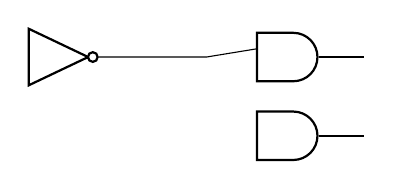
\begin{tikzpicture}[circuit logic US, every circuit symbol/.style={thick}]
	% Logic Gates
	\node[and gate,inputs={nn}, point right] (and1) at (2,-1)    {};
	\node[and gate,inputs={nn}, point right] (and2) at (2,-2)    {};
	\node[not gate, point right]               (not1) at (-1,-1) {};
	
	
	\draw (not1.output) -| (1,-1) -- (and1.input 1);
	
	%Outputs
	\draw (and1.output) [thick]-- (3,-1);
	\draw (and2.output) [thick]-- (3,-2);
	
	
	
	
	
	\end{tikzpicture}
\end{document}
	\caption{AND digital logic with inverter}
	\label{fig:andCircuit}
\end{figure}
	
	
	
	
	\begin{figure}[h]
		\centering
		z% 18W MOSFET amplifier, with npn transistor.
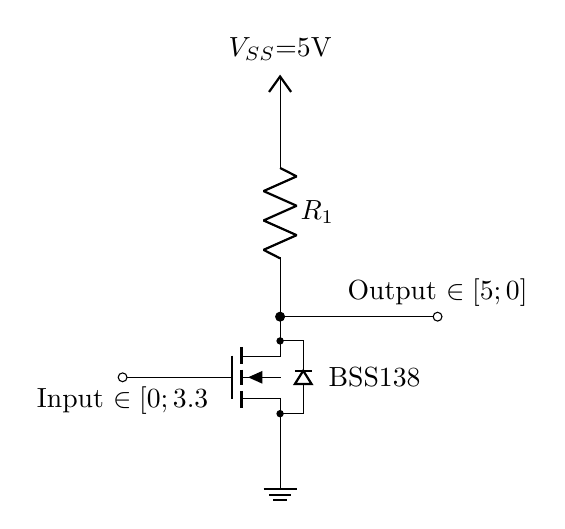
\begin{tikzpicture}[scale=2]
	\draw[color=black]
	(0,-0.5) node[ground]{}
	(0,0) node[nfet,bodydiode](npn){}
	
	(npn.B)+(0.6,0) node[]{BSS138}
	
	(0,1.7) node[vcc]{$V_{SS}$=5V}
	(0,1.7) to [R=$R_1$] (npn.D)
	(npn.S) to (0,-0.5)
	
	(-1,0) node[anchor=north]{Input $\in [0;3.3$}
	to[short,o-] (npn.G)
	
	(npn.D)+(1,0) node[anchor=south]{Output $\in [5;0]$}
	to[short,o-*]  (npn.D)
	
	
	;
	
\end{tikzpicture}

		\caption{Logic Level Converter \& Inverter Circuit}
		\label{fig:interterCirc}
	\end{figure}
	
	\subsection{JK FlipFlop's Digital Logic Circuit}
	
	\begin{figure}[h]
		\centering
		\def\JKFF(#1)#2#3{%
	\begin{scope}[shift={(#1)}]
		\draw (0,0) rectangle (1,1);
		\draw (0.5,1) -- (0.5,0);
		\draw (0.5,0.5) -- (1,0.5);
		\node at (0.75,0.75) {$Q$};
		\node at (0.75,0.25) {$\bar{Q}$};
		\draw (1,0.8) -- +(0.25,0) coordinate (#2 Q);
		\draw (0,0.2) node[right] {$K$} -- +(-0.25,0) coordinate (#2 K);
		\draw (0,0.5) node[right] {$T$} -- +(-0.25,0) coordinate (#2 T);
		\draw (0,0.8) node[right] {$J$} -- +(-0.25,0) coordinate (#2 J);
	\end{scope}
}	
	
	\begin{tikzpicture}[every path/.style={},>=triangle 45,cir1cuit logic US, every circuit symbol/.style={}]
		
		% JK FLIP FLIP LOCATION
		\JKFF(0,0){a}{$Q_0$}
		 %\draw[->] (a J) -- ++(0,1) node[left] {$+$};
		 \draw (a Q) to[short] ++(1,0) node[ocirc,label={right:DIR}] (dir) {};
		 
		% NOR GATE LOCATIONS
		\node[nor gate,inputs={nn}, point down] (nor1) at (-2,1.2) {};
		
		% NOR OUTPUT TO JK FLIPFLOP
		\draw (nor1.output) [] -- ([xshift=-1.75cm]a K) -- (a K);
		
		% XOR LOCATION
		\node[xor gate,inputs={nn}, point right] (xor1) at (0.5,2) {};
		
		% XOR OUTPUT
		\draw (xor1.output) [] -- ++(1.2,0) node[ocirc,label={right:STEP}] (step) {};
	
		% PHASE A AND PHASE B LOCATION
		\draw (-3,0)+( xor1.input 2) node[ocirc,label={left:PHASE B}] (phaseB) {};
		\draw (-3,0.2)+( xor1.input 1) node[ocirc,label={left:PHASE A}] (phaseA) {};
		
		% PHASE A to XOR GATE
		\draw[-](phaseA) -- ([xshift=-0.5cm,yshift=0.2cm] xor1.input 1) -- ([xshift=-0.5cm] xor1.input 1) -- (xor1.input 1) ;
		\draw (phaseB) -- (xor1.input 2);
		
		% CONNECTING INPUTS OF NOR GATE
		\draw[-](nor1.input 1) -- ([yshift=0.2cm]nor1.input 1) -- ([yshift=0.2cm]nor1.input 2);
		\draw[-](nor1.input 2) -- ([yshift=0.2cm]nor1.input 2);
		
		% CONNECTING PHASE A TO NOR INPUT
		\draw[-*]([xshift=0.1cm, yshift=0.2cm]nor1.input 2) -- ([xshift=0.1cm, yshift=0.88cm]nor1.input 2);
		
		% CONNECTION JK FLIPFLOP J to PHASE A
		\draw[-*](a J) -- ([xshift=-0.145cm] a J) -- ([xshift=-0.145cm,yshift=1.4cm] a J);
		
		% CONNECTION JK FLIPFLOP T to PHASE B
		\draw[-*](a T) -- ([xshift=-0.5cm] a T) -- ([xshift=-0.5cm,yshift=1.47cm] a T);
		
	%\draw[->] (a J) -- ++(0,1) node[left] {$+$};
	
	\end{tikzpicture}
		\caption{Digital Logic Circuit containing JK-Flipflops, XOR- and NOR Gates}
		\label{fig:jk_xor}
	\end{figure}
	
	The motor incremental encoder produces 2 digital signals  that has a 90 degree phase between each other shown in Figure (ref). These signals will under go a hardware filter that will produce 2 signals that indicates the direction of the motor and the incremental position. The hardware filter is implemented to reduce the processing time of the $\mu$C on the original signals.
	
	The hardware filter consist out of XOR, NOR and JK-Flipflop gates shown in Figure \ref{fig:jk_xor} and the schematic shown in Figure \ref{sch:jk_xor}. The XOR gate produces the incremental position of the motor whereas the NOR and JK-Flipflop combination produces the direction of the motor by a logical 1 or 0.
	
	%% Explain the effect of the gates maybe produce a signal table
	
	
	
	
	 These signals will be read by the $\mu$C using interrupts when a rising- \& falling edge are present.
	 
	 The encoder provides 16 lines per revolution, equal to a combined 32 rising- \& falling edges per line. The encoder provides 2 lines increasing the resolution to 64. The motor is connected to a gearbox with a reduction stage of 14:1. The encoder will thus rotate 14 times per shaft revolution, increasing the resolution to 896 per revolution.
	
	\subsection{Microcontroller}
	The microcontroller chosen is the STM32F030Mxx. The selection was done according the ease of setting up, memory size, physical dimensions and the peripherals it provided.
	
	The STM32F030MXX is based of the ARM M0 architecture which is ARM's entry level micro-controller. It requires little support to have a up and running microcontroller requiring only the SWD protocol to program and a few by-pass capacitors.
	
	It was difficult to determine the memory size specification for the project. This uncertainty ensured that the largest memory size the ARM M0 architecture could provide was selected.
	
	The Electrical and Electronic Department's Printed Circuit Board (PCB) manufacturing machine can only provide a  minimum track width \SI{0.3}{mm}. This resulted in choosing a microcontroller whose footprint would meet the requirement.
	
	Based on the conceptual design, the chosen microcontroller required to contain 2 ADC's, minimum of 5 GPIO's and 1 serial communication peripheral.
	
	
	
	
	
	\section{Verification of Model}
	%WHAT you are going to present in this chapter/section
	%WHY you are presenting it, and
	%HOW you are going to present it?
	
	The simulation is required to be a acceptable representation of the physical system to allow any further development to continue on the simulated model. It is thus important to verify whether the simulated model provides a acceptable representation of the system.
	
	
	
	

	\newpage
	%\section{Bibliography}
	\bibliographystyle{IEEEtran}
	\bibliography{IEEEabrv,references}
	
	\newpage
	\begin{appendices}
		\section{Derivation of the Double Pendulum}
		$$x_{1}= l_{1}\cos(\theta)$$
		$$y_{1} = -l_{1}\sin(\theta)$$
		
		$$x_{2} = L_{1}\sin(\theta) + l_{2}\sin(\theta + \phi)$$
		$$y_{2} = -L_{1}\cos(\theta) - l_{2}\cos(\theta + \phi)$$
		
		$$\dot{x_{2}} = L_{1}\cos(\theta)\dot{\theta} - l_{2}\cos(\theta+\phi)(\dot{\theta}+\dot{\phi}) $$
		$$\dot{y_{2}} = L_{1}\sin(\theta)\dot{\theta}+l_{2}\sin(\theta+\phi)(\dot{\theta}+\dot{\phi})$$
		
		$$x_{2}^2 = L_{1}^2\cos(\theta)^2\theta^2 +l_{2}^2\cos(\theta+\phi)^2(\dot{\theta}+\dot{\phi})^2 + 2L_{1}l_{2}\dot{\theta}(\dot{\theta}+\dot{\theta})\cos(\theta)\cos(\theta+\phi)$$
		$$y_{2}^2 = L_{1}^2\sin(\theta)^2\theta^2 +l_{2}^2\sin(\theta+\phi)^2(\dot{\theta}+\dot{\phi})^2 + 2L_{1}l_{2}\dot{\theta}(\dot{\theta}+\dot{\theta})\sin(\theta)\sin(\theta+\phi)$$
		
		$$x_{2}^2+y_{2}^2 = L_{1}^2\theta^2[\cos(\theta)^2+\sin(\theta)^2]+l_{2}^2(\dot{\theta}+\dot{\phi})^2[\cos(\theta+\phi)^2+\sin(\theta+\phi)^2] +$$
		$$ 2L_{1}l_{2}\dot{\theta}(\dot{\theta}+\dot{\phi})[\cos(\theta)\cos(\theta+\phi)+\sin(\theta)\sin(\theta+\phi)]$$	
		
		Using the following trigonometric identities $$ \cos(\gamma)^2 + \sin(\gamma)^2 = 1 $$ 
		$$ \cos(\gamma)\cos(\alpha)+\sin(\gamma)\sin(\alpha) = \cos(\gamma - \alpha) $$ the above equation resolves to: $$ V_{2}^2 = L_{1}\dot{\theta}^2+l_{2}^2(\dot{\theta}+\dot{\phi})^2 + 
		2L_{1}l_{2}(\dot{\theta}+\dot{\phi})\dot{\theta}\cos(\phi)$$
		
		The kinetic energy in the system consist of the fixed rotation of the underactuated  pendulum and the rotation and velocity of the actuated pendulum.
		
		$$ T = \frac{1}{2}I_{A}\dot{\theta}^2 + \frac{1}{2}I_{B}(\dot{\theta}+\dot{\phi})^2 + \frac{1}{2}m_{2}V_{2}^2$$
		$$ T = \frac{1}{2}I_{A}\dot{\theta}^2 + \frac{1}{2}I_{B}(\dot{\theta}+\dot{\phi})^2 + \frac{1}{2}m_{2}[L_{1}\dot{\theta}^2+l_{2}^2(\dot{\theta}+\dot{\phi})^2 + 
		2L_{1}l_{2}(\dot{\theta}+\dot{\phi})\dot{\theta}\cos(\phi)]^2$$
		
		The potential energy in the system is defined as
		$$V=-m_{1}gl_{1}\cos(\theta)-m_{2}g[L_{1}\cos(\theta)+l_{2}\cos(\theta+\phi)]$$
		
		The Lagrange is defined as 
		$$\mathcal{L}=T-V$$
		$$\mathcal{L} = \frac{1}{2}I_{A}\dot{\theta}^2 + \frac{1}{2}I_{B}(\dot{\theta}+\dot{\phi})^2 + \frac{1}{2}m_{2}[L_{1}\dot{\theta}^2+l_{2}^2(\dot{\theta}+\dot{\phi})^2 + 
		2L_{1}l_{2}(\dot{\theta}+\dot{\phi})\dot{\theta}\cos(\phi)]^2+m_{1}gl_{1}\cos(\theta)+$$
		$$m_{2}g[L_{1}\cos(\theta)+l_{2}\cos(\theta+\phi)]$$
		
		$$\frac{\partial\mathcal{L}}{\partial\theta} = -m_{1}gl_{1}\sin(\theta)-m_{2}gL_{2}\sin(\theta)-m_{2}gl_{2}\sin(\theta+\phi)$$
		$$\frac{d}{dt}\frac{\partial\mathcal{L}}{\partial\dot{\theta}} = I_{A}\ddot{\theta}+I_{B}\ddot{\theta}+I_{B}\ddot{\phi}+m_{2}L_{1}^2\ddot{\theta}+m_{2}l_{2}^2\ddot{\theta}+m_{2}l_{2}\ddot{\phi}+2m_{2}L_{1}l{2}\ddot{\theta}\cos(\phi)-2m_{2}L_{1}l_{2}\dot{\theta}\dot{\phi}\sin(\phi)+$$
		$$m_{2}L_{1}l_{2}\ddot{\phi}\cos(\phi)-m_{2}L_{1}l_{2}\dot{\phi}^2\sin(\phi)$$
		
		
		$$\frac{\partial\mathcal{L}}{\partial\phi} = -m_{2}L_{1}l_{2}(\dot{\theta}+\dot{\phi})\dot{\theta}\sin(\phi)-m_{2}gl_{2}\sin(\theta+\phi)$$
		
		$$\frac{d}{dt}\frac{\partial\mathcal{L}}{\partial\dot{\phi}}=I_{B}\ddot{\theta}+I_{B}\ddot{\phi}+m_{2}l_{2}^2\ddot{\theta}+m_{2}l_{2}^2\ddot{\phi}+m_{2}L_{1}l_{2}\ddot{\theta}\cos(\phi)-m_{2}L_{1}l_{2}\dot{\theta}\dot{\phi}\sin(\phi)$$
		
		The differential equation describing the dynamics of the system is
		$$\frac{d}{dt}\frac{\partial\mathcal{L}}{\partial\vec{\dot{q}}}-\frac{\partial\mathcal{L}}{\partial q} = B(\dot{q})+\tau(q)$$ 
		where  $ q = 
		\begin{bmatrix}
		\theta \\
		\phi
		\end{bmatrix}
		$
		
		\newpage
		\section{Linearisation of the Double Pendulum}
			
		The system will be linearised using the Taylor Series Expansion around the operating point $$ \vec{Q_{s}} = [\vec{q_{s}},\dot{\vec{q_{s}}},\ddot{\vec{q_{s}}}]^{T}=[\pi,0,0,0,0,0]$$ and approximate the system as $$F([\vec{q},\dot{\vec{q}},\ddot{\vec{q}} ]^{T}) = F(\vec{Q}) \approx F(\vec{Q_{s}})+[\Delta{\vec{Q}}\cdot\nabla F(\vec{Q_{s}})] $$
		where $\Delta{\vec{Q}} = \vec{Q} - \vec{Q_{s}} $. Resulting in 2 linear dependent equations:
		
		\begin{align}
		\Delta{\ddot{\theta}}(I_{A}+I_{B}+m_{2}l_{2}^2+m_{2}L_{1}^2+2m_{2}l_{2}L_{1})+\Delta{\ddot{\phi}(I_{B}+m_{2}l_{2}^2+m_{2}L_{1}l_{2})}+ \notag \\
		\Delta{\theta(-m_{1}gl_{1}-m_{2}gL_{1}-m_{2}gl_{2})}+\Delta{\phi(-m_{2}gl_{2})}=\Delta{\dot{\theta}}b_{1}
		\end{align}
		
		\begin{align}
		\Delta{\ddot{\theta}(I_{B}+m_{2}l_{2}^2+m_{2}L_{1}l_{2})}+\Delta{\ddot{\phi}(I_{B}+m_{2}l_{2}^2)}+\Delta{\theta(-m_{2}gl_{2})}+\notag \\ 
		\Delta{\phi(-m_{2}gl_{2})}=\tau + (\Delta{\dot{\theta}}+\Delta{\dot{\phi}})b_{2} 
		\end{align}
		
		Equation (1) and (2) can be rewritten in state-space form by substituting the 2 equations into each other to remove the angular acceleration term of the other respectable angle. 
		
		The state space variables are chosen as $\Delta{q}$ and $\Delta{\dot{q}}$ which results in the state space representation as:
		\[		
		\begin{bmatrix}
			\Delta{\dot{\theta}} \\
			\Delta{\dot{\phi}}	\\
			\Delta{\ddot{\theta}} \\
			\Delta{\ddot{\phi}}
		\end{bmatrix} 
		=
		\begin{bmatrix}
		x & x & x & x \\
		x & x & x & x \\
		0 & 0 & 1 & 0 \\
		0 & 0 & 0 & 1
		\end{bmatrix}
		\begin{bmatrix}
		\Delta{\theta}	\\
		\Delta{\phi}	\\
		\Delta{\dot{\theta}} \\
		\Delta{\dot{\phi}}
		\end{bmatrix}
		+
		\begin{bmatrix}
		0 \\
		1 \\
		0 \\
		0 \\
		\end{bmatrix}
		\tau
		\]
		\[
		\begin{bmatrix}
		\Delta{\theta}	\\
		\Delta{\phi}	\\
		\Delta{\dot{\theta}} \\
		\Delta{\dot{\phi}}
		\end{bmatrix}
		=
		\begin{bmatrix}
		1 & 0 & 0 & 0 \\
		0 & 1 & 0 & 0 \\
		0 & 0 & 1 & 0 \\
		0 & 0 & 0 & 1
		\end{bmatrix}
		\begin{bmatrix}
		\Delta{\theta}	\\
		\Delta{\phi}	\\
		\Delta{\dot{\theta}} \\
		\Delta{\dot{\phi}}
		\end{bmatrix}
		+
		\begin{bmatrix}
		0 
		\end{bmatrix}
		\tau
		\]
		
		The compact form will be used as $$ \dot{\vec{x}} = \boldsymbol{A}\vec{x} + \boldsymbol{B}\vec{u} $$ and $$ \vec{y} = \boldsymbol{D}\vec{x} + \boldsymbol{0}\vec{u} $$
		\newpage
		\section{De-coupling of the Linearised System into 2 Independent Equations}
		
		\newpage
		\section{Collocated Linearisation}
		\newpage
		\section{Proof of Pumping Energy into System}
	\end{appendices}
	
\end{document}
